\documentclass{article}

\usepackage{neurips_2026}

\usepackage[utf8]{inputenc}
\usepackage{hyperref}
\hypersetup{hidelinks}
\usepackage{url}
\usepackage{booktabs}
\usepackage{amsfonts}
\usepackage{amsmath}
\usepackage{xcolor}
\usepackage{graphicx}
\usepackage{flafter}

\title{Beyond Next-Token: Evaluating LLM Embeddings for Next-State Dynamics}

\author{%
  Anonymous Authors\\
  Anonymous Institution\\
  anonymous@example.com
}

\begin{document}

\maketitle

\begin{abstract}
Large language models are predominantly built around the next-token prediction paradigm, but many understanding and reasoning problems are more naturally viewed as next-state prediction: given a current world state and an action, a model should predict the resulting world state. Studying this paradigm requires a representation space for natural-language states. Text embedding models, which are explicitly designed to represent text as vectors, provide a natural substrate for asking whether such state representations are updateable by actions. We propose next-state vector prediction as a diagnostic evaluation for this question. Given a natural-language current state and action, we freeze the text encoder and train only a lightweight transition probe to predict the embedding of the resulting next state. The predicted vector is evaluated by whether it retrieves an equivalent next-state embedding among candidates. We build a unified evaluation suite from synthetic state changes and five public state-tracking resources—ProPara, OpenPI-C, SCONE, ALFWorld, and TRIP—and compare six encoders from five embedding families, including Qwen3-Embedding, BGE, E5, Jina, and MiniLM. Results show that frozen text embedding spaces contain usable one-step transition structure: top-1 retrieval reaches 81.4\% on OpenPI-C and 98.7\% on TRIP-known state transitions. However, row-level diagnostics and multi-step rollout reveal important limitations. Predicted vectors often land near semantically equivalent states but fail to identify the exact object or state instance, and recursively feeding predicted embeddings back into the transition model leads to rapid error accumulation. These findings suggest that current text embeddings support local one-step state-transition probes, but remain far from stable long-horizon world-state simulation.
\end{abstract}

\section{Introduction}

Language models are overwhelmingly optimized for next-token prediction. This objective has produced broadly useful representations, but it does not directly ask whether a model understands how states change. If a scene starts as ``a ball is on the table'' and the action is ``the ball is painted red,'' the desired result is not merely the next likely phrase, but the next world state: ``a red ball is on the table.'' This paper asks a simple question: can frozen text embedding spaces be used as a substrate for such next-state dynamics?

We formulate next-state prediction as a vector-valued transition problem. Given text descriptions of a current state $s_t$ and action $a_t$, we encode both with a frozen embedding model and train a small transition network $f_\theta$ to predict the embedding of the next state $s_{t+1}$. The model is trained with an InfoNCE retrieval objective, so the predicted vector must be close to the true next-state embedding and far from other next-state candidates. This framing avoids the ambiguity of surface-form text generation while preserving a concrete behavioral evaluation: whether the predicted vector retrieves the correct next state.

Our central modeling choice is a gated residual FiLM transition. Concatenating state and action vectors treats the action as another input feature. Pure FiLM modulation can be too destructive because it scales and shifts every state dimension. We therefore use the action embedding to produce feature-wise scale, shift, and gate parameters, then add a gated modulation update back to the original state:
\begin{equation}
  h_{\mathrm{mod}} = h_t + \sigma(\eta(a_t)) \odot (\gamma(a_t) \odot h_t + \beta(a_t)).
\end{equation}
This architecture expresses actions as conditional transformations while retaining a direct path for the original state and learning how strongly each dimension should be updated.

We evaluate six encoders from five embedding families: Qwen3-Embedding-0.6B and Qwen3-Embedding-8B~\citep{zhang2025qwen3embedding}, bge-large-en-v1.5~\citep{xiao2024cpack}, e5-large-v2~\citep{wang2022e5}, jina-embeddings-v3~\citep{sturua2024jinaembeddingsv3}, and all-MiniLM-L6-v2~\citep{huggingfaceAllMiniLML6V2,wang2020minilm}. We run all six encoders on the core public datasets, and use the original three encoders across the full extension suite covering procedural processes, instructional state changes, embodied household tasks, and physical commonsense stories. The resulting benchmark suite spans attribute changes, location changes, existence changes, possession, containment, heating, cooling, cleaning, opening, and object transformation.

Our contributions are:
\begin{itemize}
  \item We introduce next-state vector prediction as a direct test of whether frozen text embedding models support action-conditioned world-state dynamics.
  \item We use a lightweight gated residual FiLM transition probe trained with InfoNCE, avoiding both brittle text decoding and destructive action modulation.
\item We build a multi-dataset evaluation suite from synthetic data, ProPara, OpenPI-C, SCONE, ALFWorld, and TRIP, including natural-language rewrites for structured state annotations.
  \item We show that embedding-space transition models can perform well on several public physical-state datasets, while ALFWorld exposes a harder embodied dynamics setting.
\end{itemize}

\begin{figure}[t]
  \centering
  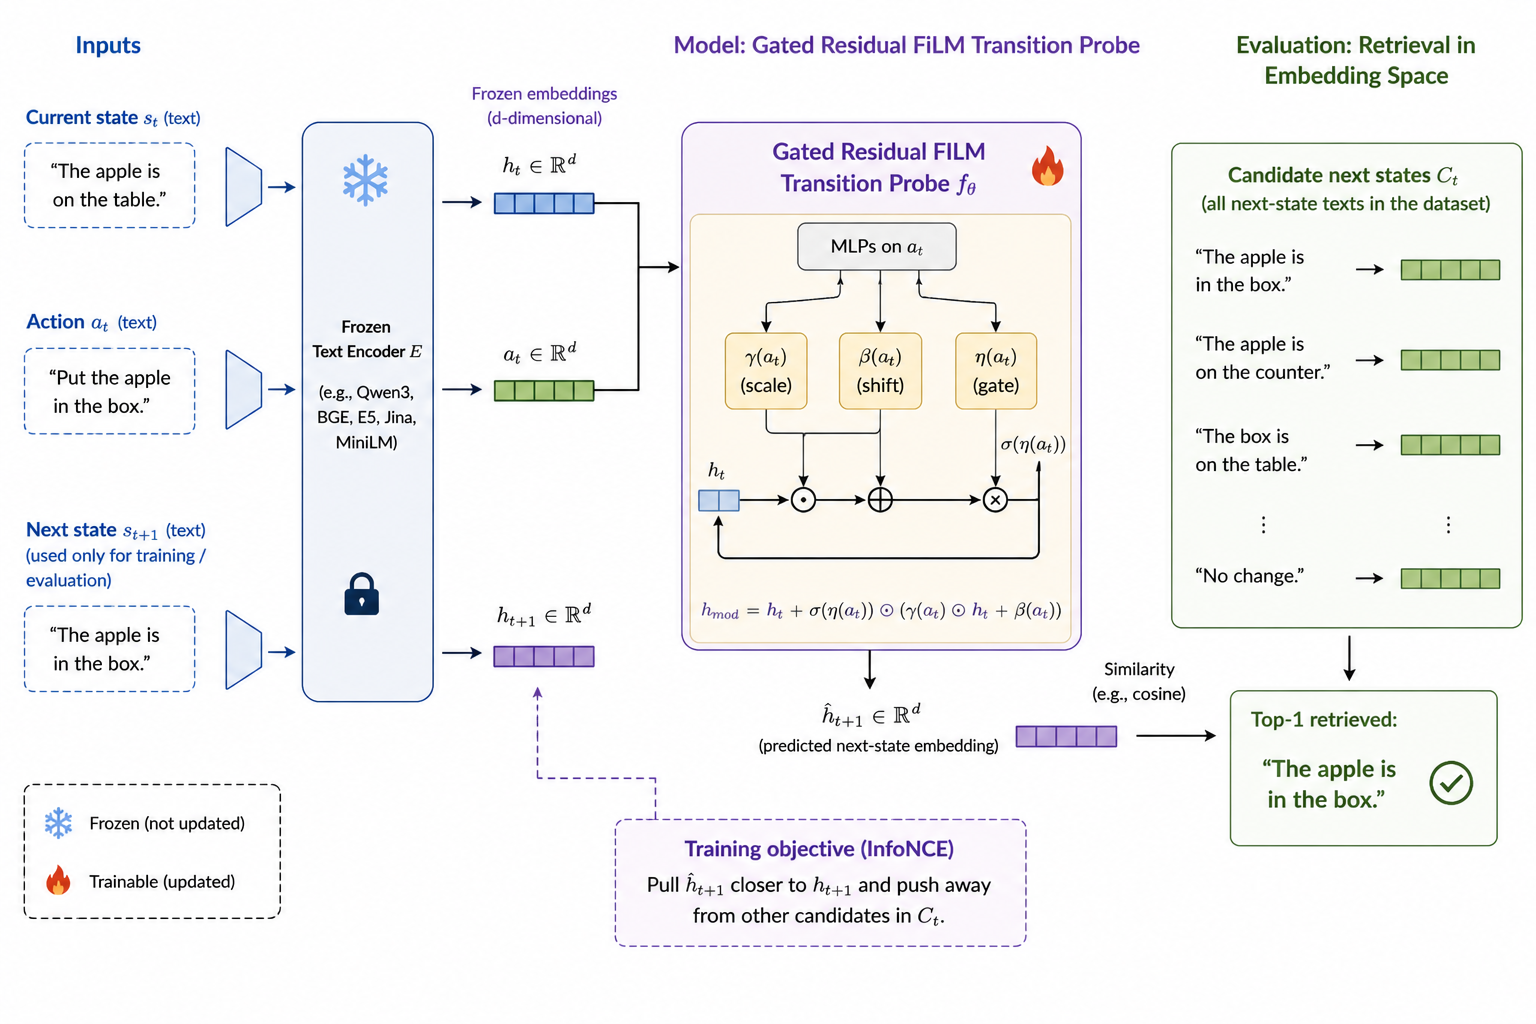
\includegraphics[width=\linewidth]{figures/figure1.png}
  \caption{Overview of next-state vector prediction. A frozen text embedding model encodes the current state and action, a lightweight transition probe predicts the next-state embedding, and retrieval evaluates whether the predicted vector recovers the correct candidate next state.}
  \label{fig:overview}
\end{figure}

\section{Related Work}

\paragraph{State tracking in language.}
Procedural and commonsense state tracking datasets evaluate whether models can follow how entities change over time. ProPara introduced paragraph-level tracking of entity existence and location in scientific processes~\citep{dalvi2018propara}. OpenPI broadened procedural tracking to open-vocabulary entity, attribute, before-state, and after-state tuples~\citep{tandon2020openpi}; OpenPI-C later cleaned this benchmark and added stronger open-vocabulary state-tracking baselines~\citep{wu2023openpic}. TRIP provides dense intuitive-physics annotations for commonsense stories and evaluates whether model predictions are supported by verifiable physical states~\citep{storks2021trip}. ALFWorld aligns text-based household games with embodied environments, yielding action traces over object locations and physical object properties~\citep{shridhar2021alfworld}. SCONE focuses on context-dependent instruction execution over symbolic worlds such as Alchemy, Scene, and Tangrams~\citep{long2016scone}, with later work studying program learning under denotation-only supervision~\citep{guu2017language}. Most prior uses of these resources cast state tracking as classification, semantic parsing, question answering, plausibility judgment, or text generation. We instead normalize them into a common vector transition format: current state, action sentence, and next state.

\paragraph{Text embeddings and retrieval models.}
Sentence embedding models turn text into fixed-dimensional vectors for semantic similarity and retrieval~\citep{reimers2019sentencebert}. We evaluate several modern open embedding families. E5 trains text embeddings with weakly supervised contrastive pre-training over large text-pair collections~\citep{wang2022e5}. BGE-large-en-v1.5 is part of the BGE/C-Pack family, which packages large-scale embedding data, benchmarks, and models and reports strong MTEB-style retrieval performance~\citep{xiao2024cpack}. Qwen3-Embedding-0.6B belongs to the Qwen3 Embedding series, which builds embedding and reranking models on top of Qwen3 foundation models with multi-stage training and synthetic data generation~\citep{zhang2025qwen3embedding}. In the later encoder sweep, we additionally evaluate jina-embeddings-v3~\citep{sturua2024jinaembeddingsv3} and all-MiniLM-L6-v2, a Sentence-Transformers model built from a compact MiniLM encoder~\citep{huggingfaceAllMiniLML6V2,wang2020minilm}. These models are usually evaluated by retrieval or semantic similarity; our question is whether their frozen geometries also support action-conditioned movement from one world-state description to another.

\paragraph{Latent dynamics and world models.}
Learning a transition function in latent space is central to world-model and model-based reinforcement-learning systems. World Models learn compact latent representations and predictive dynamics for control~\citep{ha2018worldmodels}, while Dreamer-style agents learn behaviors through latent imagination~\citep{hafner2020dreamer}. Dynalang brings this idea closer to language by learning a multimodal world model that predicts future text and image representations~\citep{lin2024dynalang}. A parallel line asks whether sequence models trained for next-token or next-move prediction acquire internal world representations, as in Othello-GPT~\citep{li2023othello}. Our work differs by explicitly training a lightweight transition operator over frozen natural-language embedding vectors rather than probing hidden activations or training an environment agent.

\paragraph{Conditional modulation and contrastive prediction.}
Our transition module is inspired by feature-wise linear modulation, which conditions neural computation through learned per-feature scale and shift parameters~\citep{perez2017film}. We adapt this mechanism to language embedding dynamics by using the action embedding to modulate the state embedding, then adding the original state back as a residual path. The training objective follows contrastive predictive coding, where future representations are predicted with an InfoNCE-style contrastive loss~\citep{oord2018cpc}. In our setting, the positives are frozen embeddings of true next states and the negatives are other next-state candidates in the minibatch.

\section{Task Formulation}

Each example is a triple $(x_t, u_t, x_{t+1})$, where $x_t$ is a natural language description of the current state, $u_t$ is a natural language action or event, and $x_{t+1}$ is the resulting state. A frozen encoder $E$ maps each text to a vector:
\begin{equation}
  h_t = E(x_t), \quad a_t = E(u_t), \quad y_t = E(x_{t+1}).
\end{equation}
The transition model predicts $\hat{y}_t = f_\theta(h_t, a_t)$. At test time, we rank candidate next-state embeddings by cosine similarity to $\hat{y}_t$. The primary metric is top-$k$ retrieval accuracy: a prediction is correct if any candidate with the same normalized next-state text is among the $k$ nearest candidates.

\section{Method}

\subsection{Gated Residual FiLM Transition Model}

Given state embedding $h_t$ and action embedding $a_t$, an action network predicts FiLM and gate parameters:
\begin{equation}
  \gamma, \beta, \eta = g_\theta(a_t).
\end{equation}
The action-conditioned state representation is:
\begin{equation}
  h_{\mathrm{mod}} = h_t + \sigma(\eta) \odot (\gamma \odot h_t + \beta).
\end{equation}
A multilayer perceptron maps $h_{\mathrm{mod}}$ to the predicted next-state vector $\hat{y}_t$, followed by $\ell_2$ normalization. The residual term gives the model a stable identity path for unchanged aspects of the state, while the gate lets the action decide how strongly to modify each embedding dimension.

\subsection{InfoNCE Objective}

For a minibatch of $B$ examples, we compute cosine similarities between each prediction $\hat{y}_i$ and each target next-state embedding $y_j$:
\begin{equation}
  \ell_i = -\log \frac{\exp(\cos(\hat{y}_i,y_i)/\tau)}
  {\sum_{j=1}^{B}\exp(\cos(\hat{y}_i,y_j)/\tau)}.
\end{equation}
The model is trained to identify the correct next state among in-batch negatives. When two minibatch examples share the same normalized next-state text, we mask the non-target copy as a false negative. This objective aligns naturally with retrieval evaluation and does not require a decoder.

\section{Datasets}

Table~\ref{tab:datasets} summarizes the datasets used in the current experimental suite. All datasets are converted into the same JSONL schema with fields \texttt{text\_t}, \texttt{action\_text}, and \texttt{text\_t1}. We globally deduplicate exact triples within each processed dataset, but retain examples that share the same next-state text while differing in the current state, action, entity, or trajectory context. During retrieval evaluation, any candidate with the same normalized next-state text as the target is counted as correct.

\begin{table}[!htbp]
  \centering
  \caption{Processed next-state datasets. Counts refer to the versions used in our experiments.}
  \label{tab:datasets}
  \small
  \setlength{\tabcolsep}{3.5pt}
  \begin{tabular}{lrrrl}
    \toprule
    Dataset & Train & Dev & Test & Notes \\
    \midrule
    Synthetic & 6000 & 800 & 1200 & Controlled attributes and relations \\
    ProPara & 2443 & 309 & 401 & Entity location/existence transitions \\
    ProPara-DeepSeek & 2443 & 309 & 401 & Natural language state rewrites \\
    OpenPI-C & 13832 & 1152 & 2030 & WikiHow procedural state changes \\
    SCONE & 55990 & 3210 & 13670 & Structured world-state transitions \\
    ALFWorld-noGoto & 18995 & 692 & 637 & Household object-state transitions \\
    TRIP-known & 2022 & 885 & 887 & Explicit known-to-known physical changes \\
    \bottomrule
  \end{tabular}
\end{table}

The synthetic split covers controlled color, size, material, temperature, switch state, wetness, containment, relative position, and room-location changes. ProPara~\citep{dalvi2018propara} is converted from entity grids into sentence-level location/existence transitions; we keep a compact template version and a DeepSeek-rewritten natural-language version. OpenPI-C~\citep{wu2023openpic} provides WikiHow before/after state changes, which we pair with the corresponding procedure step as the action.

SCONE~\citep{long2016scone} contains symbolic world-state transitions; we rewrite compact world strings into more natural descriptions before encoding them. ALFWorld~\citep{shridhar2021alfworld} contributes household actions such as pick up, put, clean, heat, cool, slice, and toggle; we remove navigation-heavy \texttt{GotoLocation} actions. TRIP~\citep{storks2021trip} contributes physical state annotations from commonsense stories, and we keep only known-to-known transitions to avoid noisy ``unknown'' targets.

Table~\ref{tab:dataset-examples} shows representative converted examples. The conversion is intentionally lightweight: each source resource is mapped into the same current-state, action, next-state interface while preserving the type of state change originally annotated by the dataset.

\begin{table}[!htbp]
  \centering
  \caption{Representative examples after conversion into the unified next-state schema. The synthetic example is shown in English for readability.}
  \label{tab:dataset-examples}
  \scriptsize
  \setlength{\tabcolsep}{2pt}
  \renewcommand{\arraystretch}{1.08}
  \begin{tabular}{p{0.15\linewidth}p{0.26\linewidth}p{0.25\linewidth}p{0.26\linewidth}}
    \toprule
    Dataset & Current state $x_t$ & Action $u_t$ & Next state $x_{t+1}$ \\
    \midrule
    Synthetic & A green coin is on the workbench. & Paint the coin black. & A black coin is on the workbench. \\
    ProPara-DeepSeek & The location of the animal's skeleton is unknown. & The animal's skeleton sinks to the bottom of an ocean. & The animal's skeleton is at the bottom of an ocean. \\
    OpenPI-C & Before the step, the temperature of mixture is cool. & In the task ``Make Ful Medames,'' perform this step: Serve hot. & After the step, the temperature of mixture is hot. \\
    SCONE & The tangram board is ordered from left to right. Position 1 has shape 1; position 2 has shape 4; position 3 has shape 0; position 4 has shape 3; position 5 has shape 2. & Switch 1st and 3rd figures. & The tangram board is ordered from left to right. Position 1 has shape 0; position 2 has shape 4; position 3 has shape 1; position 4 has shape 3; position 5 has shape 2. \\
    ALFWorld-noGoto & The lettuce is not clean. The agent is holding the lettuce. & Wash the lettuce slice in the sink and then remove it. & The lettuce is clean. The agent is holding the lettuce. \\
    TRIP-known & The pre-made breakfast sandwich is inside a container. & Tom opened the fridge and grabbed a pre-made breakfast sandwich. & The pre-made breakfast sandwich is out of a container. \\
    \bottomrule
  \end{tabular}
\end{table}

\section{Experiments}

\subsection{Main Results}

Table~\ref{tab:core-results} reports the three datasets that were run with all six encoders, so models can be compared within the same dataset group. Table~\ref{tab:extended-results} collects the remaining datasets as a separate extension set.

Across the core datasets, one-step retrieval is substantially above chance, but the difficulty varies sharply by dataset. OpenPI-C shows strong transition recoverability, while TRIP-known and ALFWorld-noGoto become very high under equivalent-next-state retrieval because many examples share the same resulting state description. Row-level diagnostic scores in Appendix~\ref{app:row-level} show that these datasets still contain substantial fine-grained instance ambiguity.

\begin{table}[t]
  \centering
  \caption{Core datasets with all six encoders using gated residual FiLM. Values are mean $\pm$ standard deviation over three seeds. Top-$k$ counts retrieval of any candidate with the same normalized next-state text as correct. Bold marks the best Top-1 encoder within each dataset group.}
  \label{tab:core-results}
  \tiny
  \setlength{\tabcolsep}{2pt}
  \begin{tabular}{llrrrr}
    \toprule
    Dataset & Encoder & Cosine & Top-1 & Top-5 & Top-10 \\
    \midrule
    OpenPI-C & \textbf{Qwen3-0.6B} & $0.532{\pm}0.001$ & $\mathbf{81.41{\pm}0.11}$ & $96.93{\pm}0.40$ & $99.16{\pm}0.15$ \\
    OpenPI-C & Qwen3-Embedding-8B & $0.488{\pm}0.008$ & $77.96{\pm}0.71$ & $95.50{\pm}0.08$ & $98.51{\pm}0.10$ \\
    OpenPI-C & jina-embeddings-v3 & $0.538{\pm}0.006$ & $75.78{\pm}0.95$ & $95.39{\pm}0.21$ & $98.29{\pm}0.23$ \\
    OpenPI-C & all-MiniLM-L6-v2 & $0.619{\pm}0.002$ & $75.16{\pm}0.53$ & $95.19{\pm}0.16$ & $98.13{\pm}0.09$ \\
    OpenPI-C & bge-large & $0.483{\pm}0.001$ & $76.11{\pm}0.23$ & $95.01{\pm}0.40$ & $97.98{\pm}0.10$ \\
    OpenPI-C & e5-large & $0.328{\pm}0.004$ & $72.46{\pm}0.81$ & $92.22{\pm}0.58$ & $96.26{\pm}0.47$ \\
    \midrule
    TRIP-known & \textbf{Qwen3-0.6B} & $0.581{\pm}0.004$ & $\mathbf{98.72{\pm}0.52}$ & $99.96{\pm}0.07$ & $100.00{\pm}0.00$ \\
    TRIP-known & Qwen3-Embedding-8B & $0.527{\pm}0.007$ & $96.54{\pm}0.43$ & $99.74{\pm}0.13$ & $99.96{\pm}0.07$ \\
    TRIP-known & jina-embeddings-v3 & $0.575{\pm}0.004$ & $97.63{\pm}0.85$ & $99.85{\pm}0.07$ & $100.00{\pm}0.00$ \\
    TRIP-known & all-MiniLM-L6-v2 & $0.717{\pm}0.001$ & $97.93{\pm}0.28$ & $99.89{\pm}0.00$ & $100.00{\pm}0.00$ \\
    TRIP-known & bge-large & $0.548{\pm}0.005$ & $98.16{\pm}0.13$ & $99.89{\pm}0.11$ & $100.00{\pm}0.00$ \\
    TRIP-known & e5-large & $0.405{\pm}0.004$ & $98.53{\pm}0.49$ & $99.85{\pm}0.07$ & $100.00{\pm}0.00$ \\
    \midrule
    ALFWorld-noGoto & Qwen3-0.6B & $0.576{\pm}0.004$ & $99.16{\pm}0.36$ & $100.00{\pm}0.00$ & $100.00{\pm}0.00$ \\
    ALFWorld-noGoto & Qwen3-Embedding-8B & $0.566{\pm}0.008$ & $99.06{\pm}0.27$ & $99.84{\pm}0.00$ & $99.90{\pm}0.09$ \\
    ALFWorld-noGoto & jina-embeddings-v3 & $0.550{\pm}0.006$ & $99.27{\pm}0.09$ & $100.00{\pm}0.00$ & $100.00{\pm}0.00$ \\
    ALFWorld-noGoto & all-MiniLM-L6-v2 & $0.671{\pm}0.006$ & $98.80{\pm}0.24$ & $99.58{\pm}0.09$ & $99.90{\pm}0.09$ \\
    ALFWorld-noGoto & \textbf{bge-large} & $0.523{\pm}0.004$ & $\mathbf{99.37{\pm}0.16}$ & $99.95{\pm}0.09$ & $99.95{\pm}0.09$ \\
    ALFWorld-noGoto & e5-large & $0.380{\pm}0.002$ & $98.90{\pm}0.42$ & $99.90{\pm}0.18$ & $100.00{\pm}0.00$ \\
    \bottomrule
  \end{tabular}
\end{table}

\subsection{Architecture Ablation}

Figure~\ref{fig:architecture-ablation} visualizes the averaged architecture trends, and Table~\ref{tab:architecture-ablation} reports the full per-encoder ablation results. We report mean top-1 retrieval over three random seeds. FiLM-style modulation improves over concatenation on most dataset--encoder pairs, with the clearest gains on OpenPI-C and TRIP-known. Adding a gate to residual FiLM often helps further, though not uniformly across all encoders. State-only is unexpectedly strong on TRIP-known, suggesting that many known-state transitions can be partially inferred from the current state distribution alone. Action-only is much weaker on OpenPI-C and TRIP-known, confirming that the action alone usually does not identify the next state. On ALFWorld-noGoto, however, action-only becomes more competitive with full transition models, suggesting that some household actions carry strong priors over the resulting object state.

\begin{figure}[t]
  \centering
  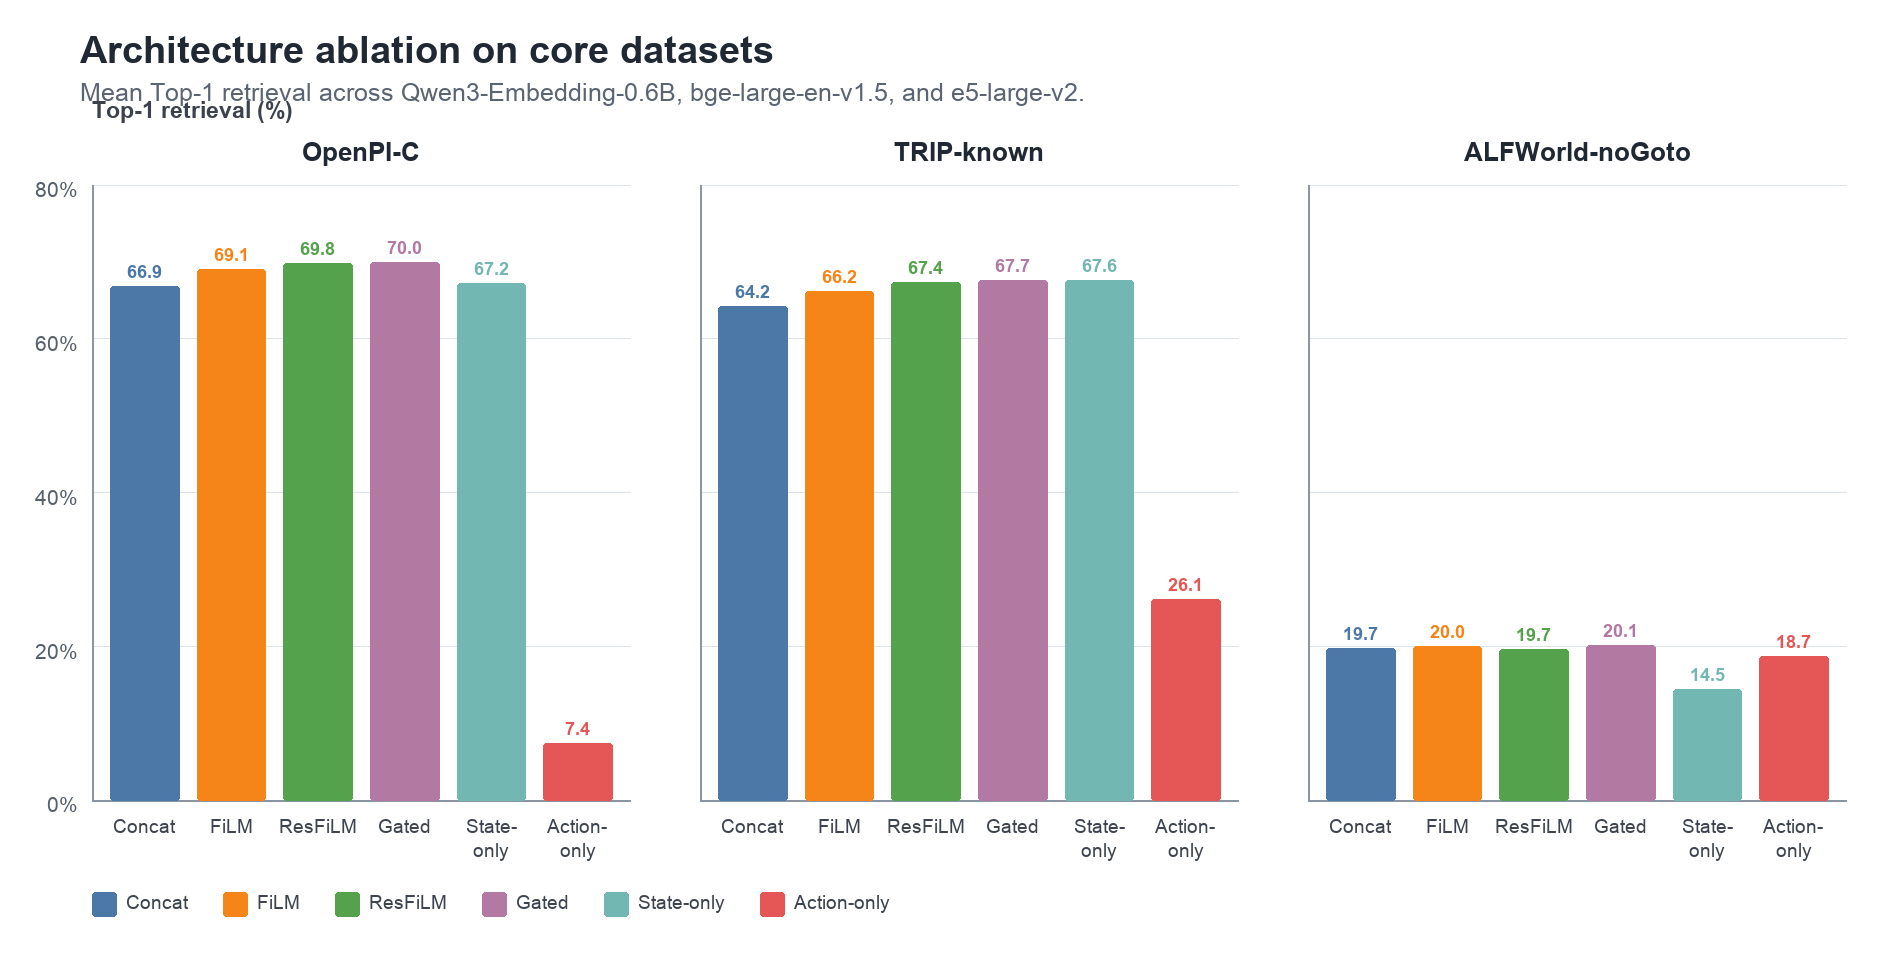
\includegraphics[width=\linewidth]{figures/architecture_ablation.png}
  \caption{Architecture ablation averaged over the original three encoders on the core datasets. Full transition models are compared with diagnostic state-only and action-only baselines.}
  \label{fig:architecture-ablation}
\end{figure}

\begin{table}[t]
  \centering
  \caption{Architecture ablation on core datasets. Values are top-1 retrieval accuracy, mean $\pm$ standard deviation over three seeds. Bold marks the best full transition model among concat, FiLM, residual FiLM, and gated residual FiLM. State-only and action-only are diagnostic input-prior baselines.}
  \label{tab:architecture-ablation}
  \tiny
  \setlength{\tabcolsep}{1.5pt}
  \begin{tabular}{llcccccc}
    \toprule
    Dataset & Encoder & Concat & FiLM & Residual FiLM & Gated ResFiLM & State-only & Action-only \\
    \midrule
    OpenPI-C & Qwen3-Embedding-0.6B & $79.26{\pm}0.45$ & $80.49{\pm}0.23$ & $80.25{\pm}0.45$ & $\mathbf{81.41{\pm}0.11}$ & $78.77{\pm}0.70$ & $8.56{\pm}0.29$ \\
    OpenPI-C & bge-large-en-v1.5 & $72.63{\pm}2.98$ & $76.08{\pm}0.62$ & $75.96{\pm}0.26$ & $\mathbf{76.11{\pm}0.23}$ & $73.46{\pm}0.79$ & $8.24{\pm}0.20$ \\
    OpenPI-C & e5-large-v2 & $66.06{\pm}0.73$ & $71.17{\pm}0.50$ & $\mathbf{72.56{\pm}0.31}$ & $72.46{\pm}0.81$ & $68.88{\pm}0.40$ & $6.44{\pm}0.92$ \\
    \midrule
    TRIP-known & Qwen3-Embedding-0.6B & $96.17{\pm}2.06$ & $97.33{\pm}0.34$ & $\mathbf{98.76{\pm}0.23}$ & $98.72{\pm}0.52$ & $98.72{\pm}0.17$ & $42.31{\pm}0.85$ \\
    TRIP-known & bge-large-en-v1.5 & $91.02{\pm}1.49$ & $94.89{\pm}1.49$ & $\mathbf{98.61{\pm}0.07}$ & $98.16{\pm}0.13$ & $96.47{\pm}1.17$ & $42.92{\pm}0.66$ \\
    TRIP-known & e5-large-v2 & $93.12{\pm}1.93$ & $96.43{\pm}1.53$ & $\mathbf{98.61{\pm}0.26}$ & $98.53{\pm}0.49$ & $98.20{\pm}0.39$ & $40.32{\pm}1.13$ \\
    \midrule
    ALFWorld-noGoto & Qwen3-Embedding-0.6B & $99.16{\pm}0.24$ & $\mathbf{99.32{\pm}0.24}$ & $99.22{\pm}0.16$ & $99.16{\pm}0.36$ & $81.84{\pm}0.09$ & $90.27{\pm}1.03$ \\
    ALFWorld-noGoto & bge-large-en-v1.5 & $99.32{\pm}0.09$ & $99.27{\pm}0.09$ & $99.27{\pm}0.24$ & $\mathbf{99.37{\pm}0.16}$ & $82.31{\pm}0.77$ & $91.58{\pm}1.27$ \\
    ALFWorld-noGoto & e5-large-v2 & $\mathbf{99.16{\pm}0.09}$ & $98.85{\pm}0.55$ & $98.95{\pm}0.33$ & $98.90{\pm}0.42$ & $82.00{\pm}0.50$ & $90.21{\pm}0.73$ \\
    \bottomrule
  \end{tabular}
\end{table}

\begin{table}[t]
  \centering
  \caption{Extension datasets with the original three encoders using gated residual FiLM. Values are mean $\pm$ standard deviation over three seeds. Bold marks the best Top-1 encoder within each dataset group.}
  \label{tab:extended-results}
  \tiny
  \setlength{\tabcolsep}{2pt}
  \begin{tabular}{llrrrr}
    \toprule
    Dataset & Encoder & Cosine & Top-1 & Top-5 & Top-10 \\
    \midrule
    ProPara & Qwen3-0.6B & $0.415{\pm}0.003$ & $41.15{\pm}0.86$ & $80.71{\pm}1.01$ & $90.69{\pm}0.29$ \\
    ProPara & \textbf{bge-large} & $0.385{\pm}0.004$ & $\mathbf{46.22{\pm}3.95}$ & $80.96{\pm}1.52$ & $91.35{\pm}0.76$ \\
    ProPara & e5-large & $0.264{\pm}0.004$ & $45.80{\pm}2.09$ & $78.64{\pm}2.88$ & $89.36{\pm}1.46$ \\
    \midrule
    ProPara-DeepSeek & \textbf{Qwen3-0.6B} & $0.427{\pm}0.009$ & $\mathbf{45.22{\pm}3.16}$ & $81.38{\pm}1.18$ & $92.44{\pm}0.94$ \\
    ProPara-DeepSeek & bge-large & $0.397{\pm}0.006$ & $41.15{\pm}1.80$ & $77.89{\pm}0.52$ & $91.27{\pm}1.98$ \\
    ProPara-DeepSeek & e5-large & $0.256{\pm}0.004$ & $38.40{\pm}2.38$ & $73.98{\pm}1.04$ & $85.12{\pm}1.87$ \\
    \midrule
    SCONE-full & \textbf{Qwen3-0.6B} & $0.324{\pm}0.001$ & $\mathbf{8.68{\pm}6.12}$ & $23.69{\pm}13.50$ & $33.39{\pm}15.56$ \\
    SCONE-full & bge-large & $0.293{\pm}0.002$ & $3.82{\pm}2.29$ & $10.70{\pm}5.92$ & $17.32{\pm}8.75$ \\
    SCONE-full & e5-large & $0.220{\pm}0.004$ & $3.64{\pm}2.29$ & $9.20{\pm}5.28$ & $14.71{\pm}7.42$ \\
    \bottomrule
  \end{tabular}
\end{table}

\subsection{Autoregressive Multi-Step Rollout}

The preceding experiments evaluate one-step transitions, where each prediction starts from a gold current-state embedding. We additionally test whether the learned transition can be rolled forward without resetting to gold states. In autoregressive rollout, the first step uses the gold initial state and action, while later steps use the previous predicted vector as the next state input. Table~\ref{tab:multistep-rollout} reports final-horizon retrieval after three or five actions. SCONE provides the most stable multi-step estimate because it has thousands of contiguous windows; ALFWorld-noGoto and ProPara-DeepSeek provide smaller but useful trajectory-style checks. Strict three-step TRIP-known filtering leaves only ten windows, so we exclude it from the main multi-step table.

As a diagnostic, we also run a teacher-forced variant on the same windows, where each step receives the gold current-state embedding rather than the previous prediction. Teacher forcing remains much stronger than autoregressive rollout: for Qwen3-Embedding-0.6B on SCONE-full, final top-10 is 33.38\% for three-step teacher forcing versus 4.99\% for three-step autoregressive rollout, and 34.87\% versus 1.08\% for five-step rollout. The same pattern appears on the smaller trajectory sets: bge-large reaches 100.00\% teacher-forced top-10 but 42.15\% autoregressive top-10 on ALFWorld-noGoto, and 89.67\% versus 69.01\% on ProPara-DeepSeek. This gap indicates that local action-conditioned transitions are learnable, but repeated vector predictions quickly drift away from the gold state manifold.

\begin{figure}[t]
  \centering
  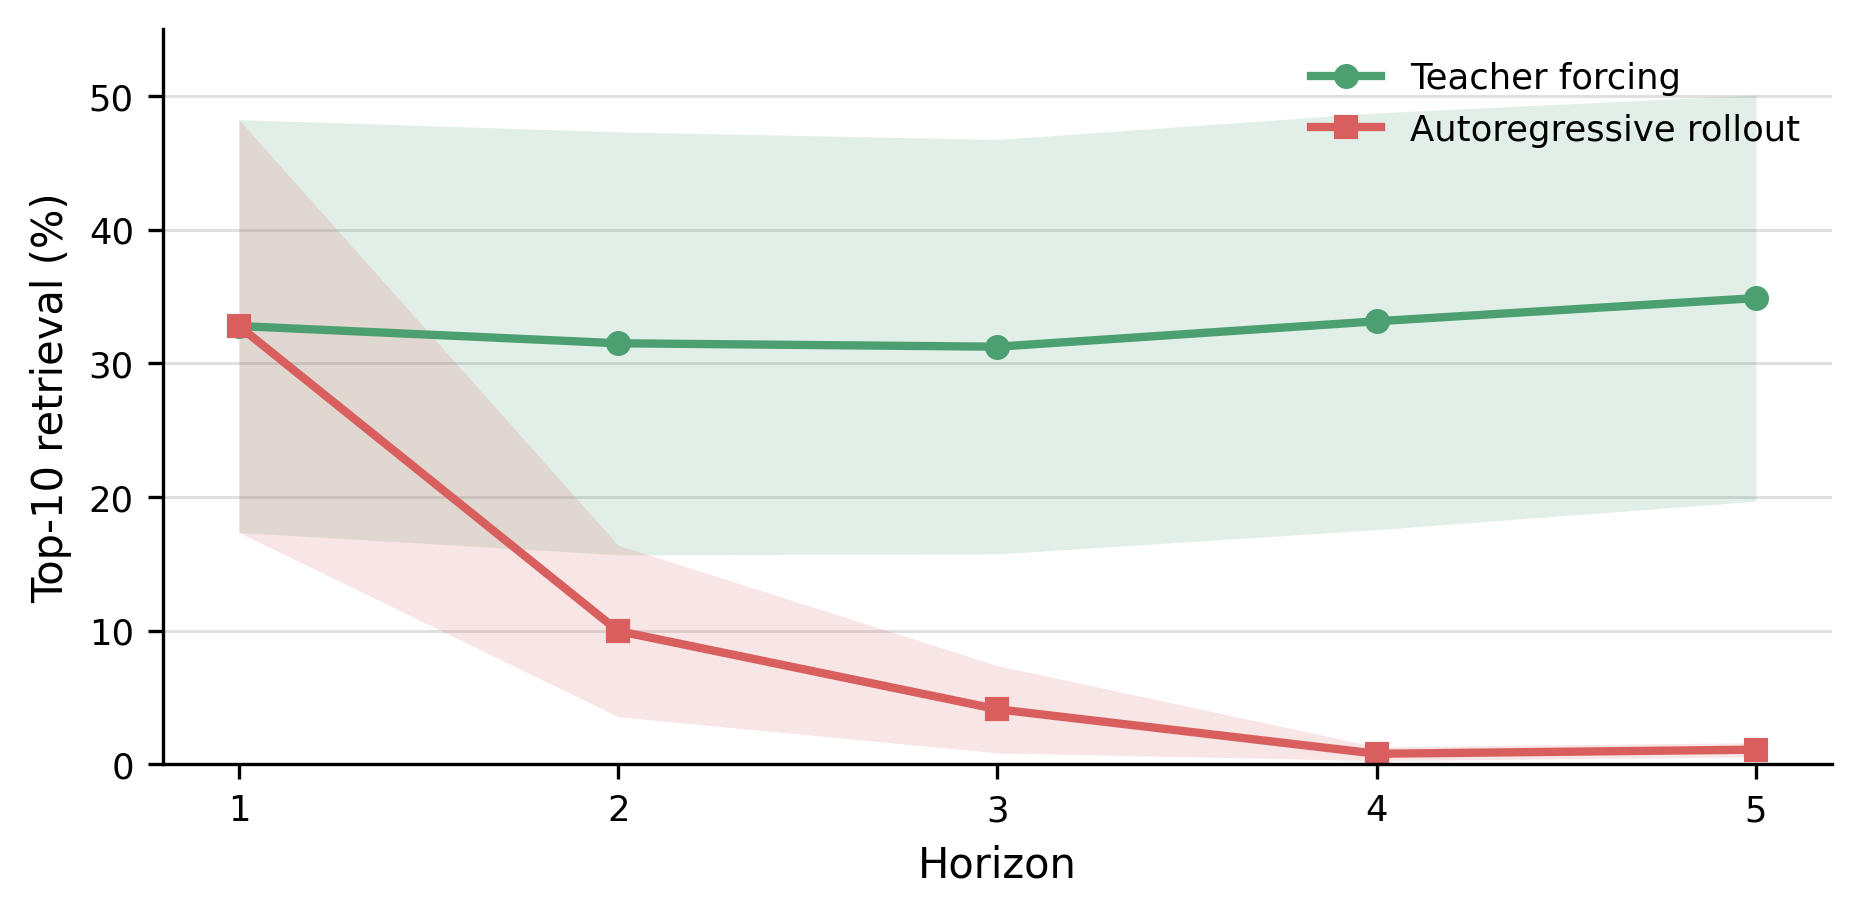
\includegraphics[width=0.88\linewidth]{figures/multistep_rollout_decay.png}
  \caption{SCONE-full multi-step Top-10 retrieval for Qwen3-Embedding-0.6B. Teacher forcing keeps each step on the gold-state manifold, while autoregressive rollout feeds predicted vectors forward and rapidly drifts.}
  \label{fig:rollout-decay}
\end{figure}

\begin{table}[t]
  \centering
  \caption{Autoregressive multi-step rollout with gated residual FiLM. Values are final-horizon top-$k$ retrieval accuracy, mean $\pm$ standard deviation over three seeds.}
  \label{tab:multistep-rollout}
  \small
  \setlength{\tabcolsep}{3.5pt}
  \begin{tabular}{lrrlrrr}
    \toprule
    Dataset & Steps & Windows & Encoder & Top-1 & Top-5 & Top-10 \\
    \midrule
    SCONE-full & 3 & 8526 & Qwen3-0.6B & $1.18{\pm}0.91$ & $3.08{\pm}2.12$ & $4.99{\pm}3.35$ \\
    SCONE-full & 3 & 8526 & bge-large & $0.42{\pm}0.27$ & $0.78{\pm}0.40$ & $1.55{\pm}0.57$ \\
    SCONE-full & 3 & 8526 & e5-large & $0.30{\pm}0.29$ & $0.82{\pm}0.64$ & $1.73{\pm}1.14$ \\
    \midrule
    SCONE-full & 5 & 3382 & Qwen3-0.6B & $0.40{\pm}0.20$ & $0.60{\pm}0.36$ & $1.08{\pm}0.53$ \\
    SCONE-full & 5 & 3382 & bge-large & $0.18{\pm}0.16$ & $0.20{\pm}0.20$ & $0.45{\pm}0.28$ \\
    SCONE-full & 5 & 3382 & e5-large & $0.17{\pm}0.12$ & $0.32{\pm}0.28$ & $0.61{\pm}0.53$ \\
    \midrule
    ALFWorld-noGoto & 3 & 189 & Qwen3-0.6B & $17.28{\pm}0.81$ & $22.22{\pm}3.30$ & $37.57{\pm}3.82$ \\
    ALFWorld-noGoto & 3 & 189 & bge-large & $17.11{\pm}2.20$ & $21.87{\pm}1.33$ & $42.15{\pm}1.62$ \\
    ALFWorld-noGoto & 3 & 189 & e5-large & $14.11{\pm}0.61$ & $17.81{\pm}0.61$ & $31.04{\pm}3.05$ \\
    \midrule
    ProPara-DeepSeek & 3 & 71 & Qwen3-0.6B & $15.96{\pm}3.54$ & $48.36{\pm}3.54$ & $69.01{\pm}2.44$ \\
    ProPara-DeepSeek & 3 & 71 & bge-large & $16.43{\pm}2.93$ & $44.60{\pm}6.35$ & $69.01{\pm}4.88$ \\
    ProPara-DeepSeek & 3 & 71 & e5-large & $8.45{\pm}1.41$ & $29.11{\pm}8.01$ & $48.36{\pm}11.98$ \\
    \bottomrule
  \end{tabular}
\end{table}

\subsection{Natural Language Rewriting}

ProPara exposes a useful preprocessing question: should structured states be kept as templates or rewritten into natural language? Rewriting improves Qwen3-Embedding-0.6B from 41.15\% to 45.22\% top-1 and improves top-10 from 90.69\% to 92.44\%. The top-1 effect is not uniform across encoders: bge decreases from 46.22\% to 41.15\%, while e5 decreases from 45.80\% to 38.40\%. This suggests that natural-language rewriting can better match some embedding spaces while introducing surface-form shifts that affect neighborhood structure.

\subsection{Dataset Difficulty}

The same model behaves very differently across datasets. TRIP-known reaches high equivalent-state retrieval despite a small training set, likely because state changes are explicit and often map cleanly onto adjective oppositions such as whole/in pieces or present/not present. ALFWorld-noGoto also has very high equivalent-state retrieval but much lower row-level retrieval in Appendix~\ref{app:row-level}, indicating that predictions land near semantically matching states while often failing to identify the exact object/action instance. This is a useful failure mode for future work: embedding geometry captures coarse transition type but blurs fine-grained household entities and repeated object states.

\paragraph{Rollout error accumulation.}
Multi-step rollout reveals a sharper limitation than one-step retrieval. On SCONE-full, Qwen3-Embedding-0.6B falls from 8.68\% one-step top-1 on all test transitions to 1.18\% after three autoregressive steps and 0.40\% after five. This indicates that the model can learn local vector transitions but does not yet preserve enough state information for reliable long-horizon dynamics.

\section{Analysis}

\paragraph{Which attributes are easy?}
On TRIP-known, object attributes such as mixed, edible, functional, running, pieces, and location are typically easier than human location. For Qwen3, top-1 reaches 75.0\% on object location, 78.4\% on existence, 81.3\% on functional, 85.7\% on edible, and 92.9\% on mixed, but only 11.5\% on human location. Human movement annotations are often generic, e.g., ``Tom is in one location'' to ``Tom is in a new location,'' creating many near-identical candidates.

\paragraph{Embedding model differences.}
The best encoder depends on the dataset: Qwen3-Embedding-0.6B is strongest on OpenPI-C and TRIP-known, while bge-large-en-v1.5 is strongest on ALFWorld-noGoto and ProPara. Cosine alignment and retrieval are related but not identical; for example, all-MiniLM-L6-v2 has high cosine on TRIP-known but does not yield the best top-1 retrieval. These differences matter because the transition model is trained on top of a frozen geometry; the downstream difficulty depends on how each encoder separates fine-grained state descriptions.

\paragraph{Qualitative failure modes.}
Inspection of top-1 retrieval errors shows that the most meaningful failures are not random mismatches. On OpenPI-C, predictions often identify the correct entity and attribute but choose a nearby value, e.g., hot versus boiling or smooth versus smoother, or confuse adjacent schema fields such as wetness and moisture. On ALFWorld-noGoto, the model usually recovers the coarse household effect, such as placing an object into a receptacle, but selects the wrong instance, e.g., shelf versus bowl or cabinet versus drawer. SCONE errors are dominated by long structured states with high lexical overlap: the prediction may preserve most of the board or beaker description while changing the wrong position, color, or quantity. ProPara failures more often involve entity lifecycle changes, such as failing to infer that a seed is no longer present after it sprouts, or that water disappears after being squeezed from peat. These patterns suggest that frozen text embeddings support coarse transition type, but still struggle with fine-grained variable binding and lifecycle updates.

\paragraph{Why gated residual FiLM?}
Our ablations indicate that action-conditioned modulation is useful, but pure modulation risks erasing the original state. The gated residual FiLM design keeps $h_t$ available while allowing action-specific feature shifts and learning the update strength per dimension. This is especially important for next-state prediction, where many aspects of the state remain unchanged.

\section{Limitations}

This is an embedding-space study rather than a full language generation system. Retrieval metrics show whether the predicted vector identifies an equivalent next-state candidate, but they do not directly measure whether a decoder could verbalize a new unseen state. Some processed datasets rely on templated conversions from structured annotations, and natural-language rewriting can introduce subtle semantic drift. Row-level diagnostics remain conservative when multiple transitions share the same next-state text, so we report them separately in the appendix rather than using them as the main semantic retrieval metric. Several attribute categories and multi-step trajectory windows have small test counts, so fine-grained breakdowns should be interpreted cautiously. Finally, our rollout experiments cover short horizons only; longer-horizon planning or closed-loop text generation requires separate evaluation.

\section{Conclusion}

We presented next-state vector prediction as a way to test whether frozen text embedding models support action-conditioned state dynamics. A lightweight gated residual FiLM model trained with InfoNCE can learn meaningful transitions across procedural, instructional, embodied, and commonsense datasets. The results suggest that text embedding spaces encode useful latent structure for physical state change, but also show that row-level instance recovery and multi-step rollout remain difficult when many candidate states are semantically close. Moving beyond next-token prediction toward next-state dynamics offers a promising route for evaluating and improving language models as representations of changing worlds.

\bibliographystyle{plainnat}
\bibliography{references}

\appendix

\section{Reproducibility Details}
\label{app:row-level}

\paragraph{Training details.}
All transition heads are trained on frozen encoder outputs; no embedding model parameters are updated. Unless otherwise stated, we train for at most 30 epochs with early stopping patience 5 on dev cosine similarity. We use AdamW with learning rate $10^{-3}$, weight decay $10^{-4}$, dropout 0.05, hidden dimension 1024, train batch size 256, evaluation batch size 512, embedding batch size 64, and InfoNCE temperature $\tau=0.05$. We run three seeds, 20260504, 20260505, and 20260506, for the official gated residual FiLM results. Embeddings are $\ell_2$-normalized for retrieval evaluation, and top-$k$ metrics rank the predicted vector against all candidate next-state embeddings in the corresponding test split.

\paragraph{Duplicate next states.}
We remove exact duplicate triples $(x_t,u_t,x_{t+1})$ during preprocessing, but do not collapse examples that share the same next-state text while differing in current state, action, entity, or trajectory context. The main retrieval metric treats any candidate with the same normalized next-state text as correct, and InfoNCE training masks same-next-state examples in a minibatch as false negatives. We also report row-level retrieval in Table~\ref{tab:row-level-diagnostic}, where only the original test row is counted as correct.

\begin{table}[h]
  \centering
  \caption{Row-level diagnostic Top-1 compared with the main equivalent-next-state Top-1 metric. Values are mean $\pm$ standard deviation over three seeds for gated residual FiLM.}
  \label{tab:row-level-diagnostic}
  \tiny
  \setlength{\tabcolsep}{3pt}
  \begin{tabular}{llrr}
    \toprule
    Dataset & Encoder & Row-level Top-1 & Main Top-1 \\
    \midrule
    OpenPI-C & Qwen3-0.6B & $74.84{\pm}0.12$ & $81.41{\pm}0.11$ \\
    OpenPI-C & Qwen3-Embedding-8B & $71.30{\pm}0.95$ & $77.96{\pm}0.71$ \\
    OpenPI-C & jina-embeddings-v3 & $69.36{\pm}0.94$ & $75.78{\pm}0.95$ \\
    OpenPI-C & all-MiniLM-L6-v2 & $68.95{\pm}0.17$ & $75.16{\pm}0.53$ \\
    OpenPI-C & bge-large & $69.49{\pm}0.47$ & $76.11{\pm}0.23$ \\
    OpenPI-C & e5-large & $66.09{\pm}1.01$ & $72.46{\pm}0.81$ \\
    \midrule
    TRIP-known & Qwen3-0.6B & $67.76{\pm}0.98$ & $98.72{\pm}0.52$ \\
    TRIP-known & Qwen3-Embedding-8B & $66.37{\pm}0.28$ & $96.54{\pm}0.43$ \\
    TRIP-known & jina-embeddings-v3 & $67.94{\pm}0.62$ & $97.63{\pm}0.85$ \\
    TRIP-known & all-MiniLM-L6-v2 & $67.38{\pm}0.56$ & $97.93{\pm}0.28$ \\
    TRIP-known & bge-large & $67.83{\pm}0.58$ & $98.16{\pm}0.13$ \\
    TRIP-known & e5-large & $68.62{\pm}0.23$ & $98.53{\pm}0.49$ \\
    \midrule
    ALFWorld-noGoto & Qwen3-0.6B & $17.84{\pm}2.43$ & $99.16{\pm}0.36$ \\
    ALFWorld-noGoto & Qwen3-Embedding-8B & $18.47{\pm}0.50$ & $99.06{\pm}0.27$ \\
    ALFWorld-noGoto & jina-embeddings-v3 & $19.57{\pm}1.18$ & $99.27{\pm}0.09$ \\
    ALFWorld-noGoto & all-MiniLM-L6-v2 & $18.42{\pm}1.89$ & $98.80{\pm}0.24$ \\
    ALFWorld-noGoto & bge-large & $20.20{\pm}0.40$ & $99.37{\pm}0.16$ \\
    ALFWorld-noGoto & e5-large & $20.57{\pm}0.72$ & $98.90{\pm}0.42$ \\
    \midrule
    ProPara & Qwen3-0.6B & $32.59{\pm}0.38$ & $41.15{\pm}0.86$ \\
    ProPara & bge-large & $36.91{\pm}3.26$ & $46.22{\pm}3.95$ \\
    ProPara & e5-large & $36.16{\pm}1.52$ & $45.80{\pm}2.09$ \\
    \midrule
    ProPara-DeepSeek & Qwen3-0.6B & $41.15{\pm}3.36$ & $45.22{\pm}3.16$ \\
    ProPara-DeepSeek & bge-large & $38.15{\pm}1.52$ & $41.15{\pm}1.80$ \\
    ProPara-DeepSeek & e5-large & $35.16{\pm}2.13$ & $38.40{\pm}2.38$ \\
    \midrule
    SCONE-full & Qwen3-0.6B & $6.20{\pm}4.54$ & $8.68{\pm}6.12$ \\
    SCONE-full & bge-large & $2.29{\pm}1.38$ & $3.82{\pm}2.29$ \\
    SCONE-full & e5-large & $2.16{\pm}1.30$ & $3.64{\pm}2.29$ \\
    \bottomrule
  \end{tabular}
\end{table}

\paragraph{Reproducibility package.}
The anonymous supplemental package includes preprocessing, training, evaluation, and aggregation scripts, model-configuration templates, processed split metadata, and result-summary tables. The experiments can be reproduced from regenerated processed JSONL splits and scripts used to encode frozen embeddings, train the transition heads, and evaluate one-step and multi-step retrieval. The main scripts are the next-state vector prediction trainer and the autoregressive/teacher-forced rollout evaluator; processed files use the common fields \texttt{text\_t}, \texttt{action\_text}, and \texttt{text\_t1}. The official tables are generated from per-seed CSV summaries and then aggregated into mean and standard deviation tables.

\paragraph{Compute resources.}
Experiments were run on a cloud GPU workstation with an NVIDIA RTX 4090D GPU with 24GB memory, CPU workers, and local SSD storage for embedding caches. Large encoder sweeps were run as independent jobs over dataset--encoder--seed combinations, with embedding caches reused across architecture and rollout evaluations. Once frozen embeddings are cached, each transition-probe run takes roughly 10--100 seconds depending on dataset and encoder; the logged probe-training suites total about 1--2 single-GPU hours. End-to-end reproduction including first-time embedding extraction requires several single-GPU hours. The reported results require substantially less compute than full LLM fine-tuning because all encoders are frozen and only lightweight transition heads are trained.

\section{Asset and Dataset Documentation}

\paragraph{Dataset documentation.}
All processed examples use the JSONL schema \texttt{text\_t}, \texttt{action\_text}, and \texttt{text\_t1}. Table~\ref{tab:datasets} reports train/dev/test sizes. Section 5 describes the source and conversion procedure for each dataset. The processed splits are derived from public datasets and should be used under the licenses and terms of the original sources. We do not collect new human-subject data.

\begin{table}[h]
  \centering
  \caption{Existing assets used in the experiments. License entries reflect the official repository, project page, Hugging Face model card, or dataset card metadata checked for the assets we used.}
  \label{tab:asset-licenses}
  \footnotesize
  \setlength{\tabcolsep}{3pt}
  \begin{tabular}{p{0.24\linewidth}p{0.22\linewidth}p{0.44\linewidth}}
    \toprule
    Asset & Use & License or terms noted \\
    \midrule
    ProPara & Source dataset & Apache-2.0 \\
    OpenPI-C & Source dataset & MIT \\
    ALFWorld & Source dataset & MIT; dependencies include TextWorld MIT and Fast Downward GPLv3 \\
    SCONE & Source dataset & CC-BY-SA-4.0 \\
    TRIP & Source dataset & Not specified in official Hugging Face dataset card or GitHub metadata \\
    Qwen3-Embedding-0.6B/8B & Frozen encoder & Apache-2.0 \\
    bge-large-en-v1.5 & Frozen encoder & MIT \\
    e5-large-v2 / multilingual-e5-large & Frozen encoder & MIT \\
    jina-embeddings-v3 & Frozen encoder & CC-BY-NC-4.0 \\
    all-MiniLM-L6-v2 & Frozen encoder & Apache-2.0 \\
    \bottomrule
  \end{tabular}
\end{table}

For assets whose license is not clearly specified in the checked public metadata, we use them only for research evaluation in this submission and will verify redistribution permissions before releasing processed derivative files.

\section{Broader Impacts}

This work is primarily an evaluation and modeling study of frozen language embeddings for state transition prediction. A positive impact is that it may provide a more direct way to evaluate whether language representations encode changes in the world, which could improve diagnostics for procedural reasoning, instruction following, and embodied language systems. Potential negative impacts are indirect: better state tracking could be incorporated into systems that plan or monitor actions, and errors in predicted state dynamics could be harmful if used without verification in high-stakes settings. We therefore frame the method as a retrieval-based research benchmark rather than a deployment-ready decision system.

\input{checklist}

\end{document}
